%**************************************************************
\section{Il paradigma imperativo: il framework Qt in C++}
\label{sec:paradigma-imperativo-qt-cpp}

\emph{Qt} è uno dei \gls{frameworkg} più conosciuti per l'implementazione di applicazioni con interfacce grafiche usando il linguaggio C++.\\
Come in \emph{Flutter}, anche in \emph{Qt} le componenti grafiche si chiamano widget, e rappresentano le componenti native disponibili nel sistema in cui viene sviluppata l'applicazione (pulsanti, menu, caselle di testo, ecc.).\\
Esiste in \emph{Qt} un altro modo di rappresentare un'interfaccia grafica, chiamata \emph{QML}, ma non è scopo di questo capitolo e di questo documento introdurla.\\
\textbf{N.B.} L'implementazione dell'esempio non viene fatta seguendo le \gls{bestpracticeg} di \emph{Qt} e C++, è semplicemente il minimo essenziale per avere un applicazione funzionante col minor codice sorgente possibile.

\subsection{Creazione dell'interfaccia grafica}
\label{subsec:creazione-ui-qt}

Per implementare l'esempio indicato in "\hyperref[sec:introduzione-esempio-confronto-paradigmi]{Introduzione all'esempio per il confronto}", sono necessari pochi widget: una finestra e un pulsante, rispettivamente un \emph{QWidget} e un \emph{QPushButton}.
\begin{lstlisting}
#include <cstdlib>
#include <string>
#include <QWidget>
#include <QPushButton>
#include <QApplication>
#include <QString>

using std::to_string;

// Widget che definisce i dettagli della schermata
// e come comportarsi.
class ExampleApp : public QWidget {
  Q_OBJECT
  public:
    // Costruttore
    explicit ExampleApp(QWidget* parent = 0): QWidget(parent) {    
      // Impostazione di una dimensione fissa
      // per la finestra.
      setFixedSize(150, 100);
        
      // Prima generazione del numero casuale.
      r = rand() % 10;
        
      // Creazione del pulsante e impostazioni
      // per il suo funzionamento.
      button = new QPushButton(QString::fromStdString("Generato: " + to_string(r)), this);
      button->setCheckable(true);
      button->show();
        
      // Collegamento alla gestione degli eventi:
      // il SIGNAL descrive l'evento, la pressione del pulsante e
      // lo SLOT descrive cosa fare alla pressione del pulsante.
      connect(button, SIGNAL(clicked(bool)), this, SLOT(buttonClicked(bool)));
    };

    // Distruttore
    virtual ~ExampleApp() {};
    
  private slots:
    // Gestore dell'evento "Pressione del pulsante"
    void buttonClicked(bool _) {
      r = rand() % 10;
      button->setText(QString::fromStdString("Generato: " + to_string(r)));
    };
  private:
    int r;
    QPushButton* button;
};
\end{lstlisting}
Riassumendo, nella classe \texttt{ExampleApp}, che estende \texttt{QWidget}, viene:
\begin{itemize}
    \item definita la schermata stessa, impostando delle dimensioni fisse;
    \item generato il valore di $r$ iniziale e assegnato all'etichetta del pulsante nella sua creazione;
    \item impostato che il pulsante è cliccabile e reso visibile;
    \item connesso esplicitamente l'evento\footnote{Ciò che nella programmazione ad eventi è chiamato \emph{evento}, in \emph{Qt} è chiamato \emph{signal}.} \emph{clicked} con il \emph{callback} definito a livello di classe \texttt{buttonClicked}.
\end{itemize}
Quello che succede alla pressione del pulsante è la generazione di un evento \emph{clicked} e l'esecuzione del \emph{callback} \texttt{buttonClicked} che, avendo il riferimento al pulsante, ne imposta esplicitamente la nuova etichetta.

\subsection{Creazione del punto di ingresso}
\label{subsec:creazione-main-qt}

Definita \texttt{ExampleApp}, va definita la funzione \texttt{main}, il punto d'ingresso del programma:
\begin{lstlisting}
#include "ExampleApp.h"

// Main in cui viene avviato il programma e la schermata.
int main(int argc, char** argv) {
  // Inizializzazione schermata Qt.
  QApplication app(argc, argv);

  // Creazione della finestra.
  ExampleApp* exampleApp = new ExampleApp();
  exampleApp->show();

  return app.exec();
}
\end{lstlisting}
Quello che avviene in questo \texttt{main} è molto semplice: viene istanziato un oggetto di \texttt{QApplication}, che è un manager dell'interfaccia grafica in \emph{Qt}, e viene dichiarata un'istanza di \texttt{ExampleApp}, successivamente visualizzata tramite il metodo \texttt{show}.\\
L'applicazione realizzata è la seguente:
\begin{figure}[!h] 
  \centering 
  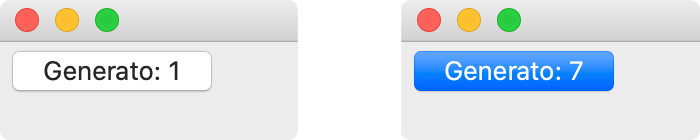
\includegraphics[width=1.0\columnwidth]{capitolo-5/qt} 
  \caption{Esempio in \emph{Qt} - Applicazione prima (sinistra) e dopo (destra) la pressione del pulsante}
\end{figure}

\subsection{Osservazioni sul procedimento}
\label{subsec:osservazioni-procedimento-qt}

Quello che si vuole evidenziare utilizzando \emph{Qt} come esempio non sono tanto le classi da usare o le necessità del linguaggio su cui si basa il \gls{frameworkg}, bensì come un'operazione di cambio dello stato dell'applicazione venga eseguita ed il ragionamento dietro ad essa.\\
Con questo tipo di \textbf{approccio imperativo}, lo sviluppatore non solo deve occuparsi dello stato dell'applicazione, ma anche dell'interfaccia grafica. Infatti nelle righe 42-43 di \texttt{ExampleApp}, una volta aggiornato $r$, lo stato, si è dovuto aggiornare il contenuto visualizzato dal pulsante tramite il metodo \texttt{setText} di \texttt{QPushButton}.